\chapter{Datasets}

This chapter presents an overview of available datasets suitable for human pose estimation in depth images. The datasets are evaluated according to closeness to real-world conditions, the amount of data and the accuracy of the recorded poses.

\section{Requirements/Considerations}

\section{Existing Datasets}

The sequences in the dataset were recorded at approximatley 30 fps. All frames and world coordinate positions at an approximate single timestep is hereby referred to as a \emph{frame}. To create samples, frames from the sequences were extracted at a set of different rates according to the amount of movement in the sequence. For sequences with a lot of movement the rate was set to every 5 seconds, moderate movement every 15 seconds, and for sequences where the subjects stood largely still, samples were extracted every 30 seconds. Each sequence is recorded by 10 different kinects from a height of 1 and 2 meters above ground. This results in a total number of 10x the amount of samples listed in Table~\ref{tab:sequences}.

\begin{figure}
  \centering
  \begin{subfigure}{.6\textwidth}
    \centering
    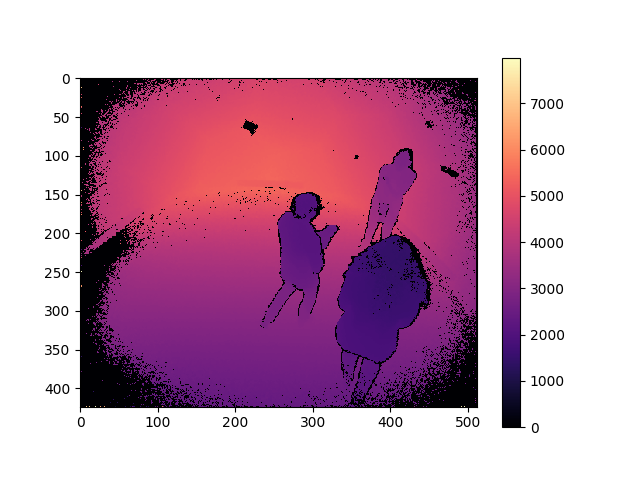
\includegraphics[width=\linewidth]{img/depth_image}
    \caption{Depth image from \texttt{KINECTNODE6}.}
    \label{fig:depth_image}
  \end{subfigure}% 
  \begin{subfigure}{.4\textwidth}
    \centering
    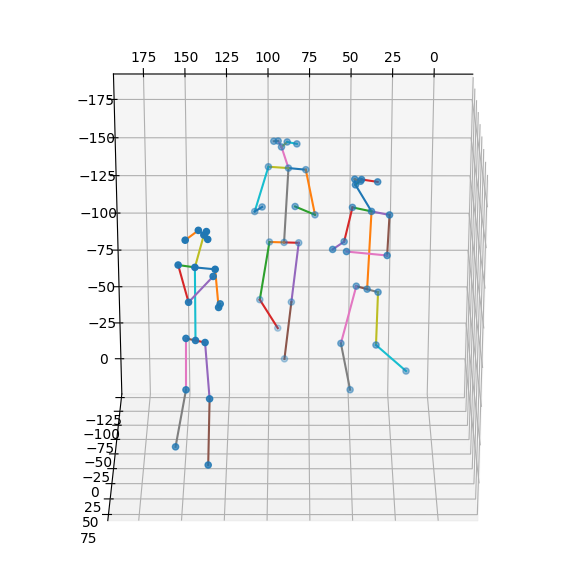
\includegraphics[width=\linewidth]{img/dataset_skeletons}
    \caption{Skeletons defined in the world coordinate system.}
    \label{fig:dataset_skeletons}
  \end{subfigure}%
  \newline
  \begin{subfigure}{.7\textwidth}
    \centering
    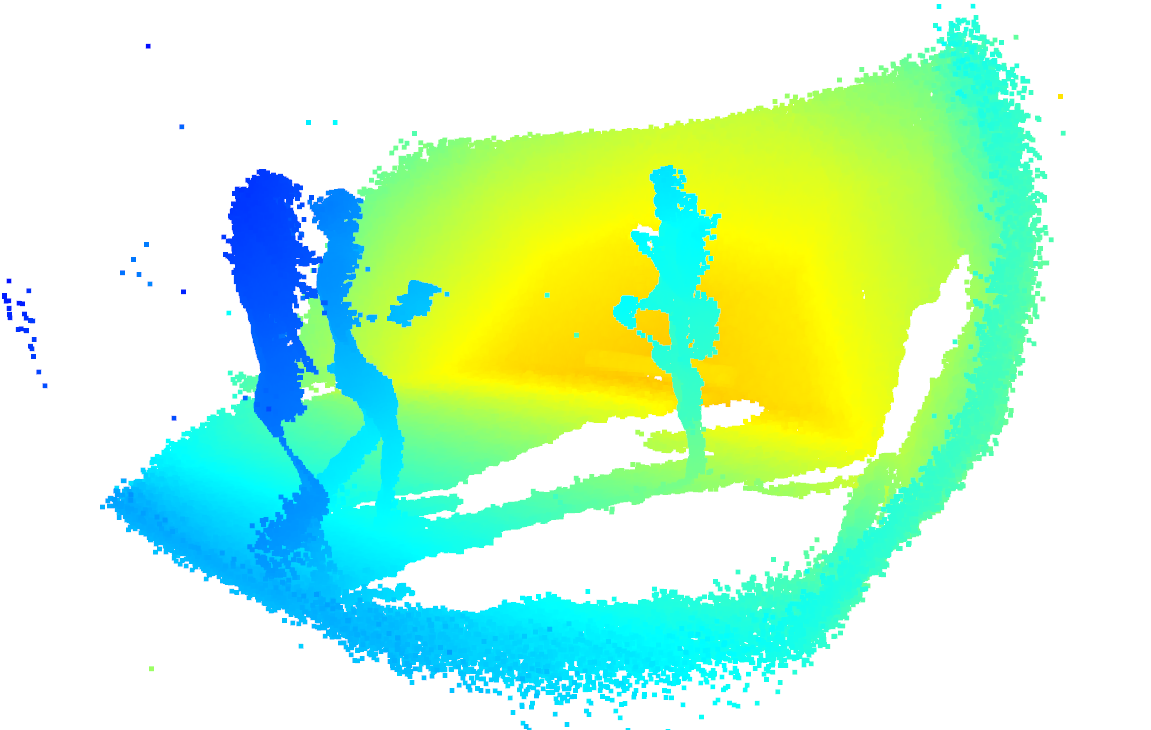
\includegraphics[width=\linewidth]{img/pointcloud}
    \caption{The depth image projected to a point cloud.}
    \label{fig:dataset_skeletons}
  \end{subfigure}%  
  \caption{Combination of datapoints for frame 144 in \cite{Joo_2015_ICCV}}
  \label{fig:skeleton_depth_duo}
\end{figure}

The dataset used in this work was created from source material provided by the Panoptic Studio \cite{Joo_2015_ICCV, Joo_2017_TPAMI}. Calibration files, predicted ground-truth skeletons and depth images were downloaded using the GNU parallel program~\cite{Tange2011a}. Some problems were experienced, as the Panoptic Studio server was quite unreliable, which resulted in significant delays, as well as corrupted files and in return a smaller dataset than desired.

A set of five complete sequences were set aside as the test set to ensure that the network wouldn't recognize any similar frames or body positions from previous sets.

\begin{table}
  \centering
  \begin{tabular}[h]{|c|l l c|}
    \hline
    & Category & Sequence Name & Duration (MM:SS) \\ \hline
    \multirow{17}{*}{\rotatebox[origin=c]{90}{Training / Validation}}
    & Range of Motion & 171204\_pose1 & 17:30 \\
    & Range of Motion & 171204\_pose2 & 22:30 \\
    & Range of Motion & 171204\_pose3 & 5:00 \\
    & Range of Motion & 171204\_pose5 & 15:00 \\ 
    & Range of Motion & 171204\_pose6 & 12:50 \\
    & Range of Motion & 171026\_pose1 & 13:20 \\
    & Range of Motion & 171026\_pose3 & 4:20 \\
    & Social Games & 160226\_haggling1 & 8:00 \\
    & Social Games & 160422\_haggling1 & 8:00 \\
    & Social Games & 160422\_ultimatum1 & 15:00 \\ 
    & Musical Instruments & 160906\_band1 & 1:00 \\ 
    & Musical Instruments & 160906\_band2 & 5:00 \\ 
    & Musical Instruments & 160906\_band3 & 5:00 \\ 
    & Toddler & 160906\_ian2 & 5:00 \\ 
    & Others & 170915\_office1 & 3:00 \\ 
    & Others & 160906\_pizza1 & 5:00 \\ 
    & Dance & 170307\_dance5 & 6:40 \\ \hline
    \multirow{5}{*}{\rotatebox[origin=c]{90}{Test}}
    & Range of Motion & 171204\_pose4 & 17:30 \\ 
    & Range of Motion & 171026\_pose2 & 9:00 \\ 
    & Social Games & 160224\_haggling1 & 5:00 \\ 
    & Toddler & 160906\_ian1 & 2:00 \\ 
    & Others & 170407\_office2 & 3:00 \\ \hline
  \end{tabular}
  \caption{Sequences used for training, validation and testing}
  \label{tab:sequences}
\end{table}


\section{Dataset Augmentations}

\begin{figure}
  \centering
  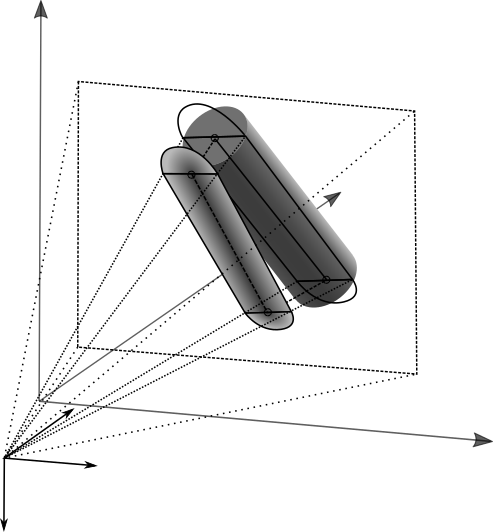
\includegraphics[width=.6\textwidth]{img/projection}
  \caption[Projection]{A limb is projected onto the image plane}
  \label{fig:projection}
\end{figure}

\begin{equation}
  \label{eq:epanechnikov}
  K(x, y) =
  \begin{cases}
    \frac{2}{\pi\sigma^{2}}(1 - ((\frac{x}{\sigma})^{2} + (\frac{y}{\sigma})^{2}) & \text{if } |(\frac{x}{\sigma})^{2} + (\frac{y}{\sigma})^{2}| \leq 1\\
    0 & \text{otherwise}
    \end{cases}
\end{equation}

\begin{figure}
  \centering
  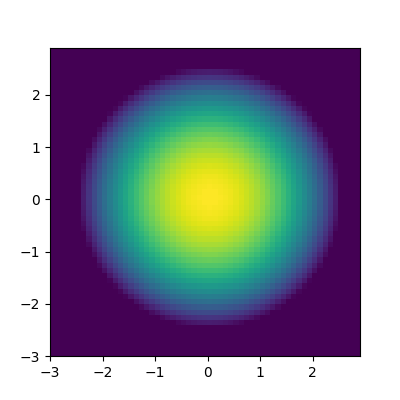
\includegraphics[width=.4\textwidth]{img/epanechnikov_2d}
  \caption{A 2D Epanechnikov \cite{epanechnikov_1969} kernel}
  \label{fig:epanechnikov}
\end{figure}

Target limb-maps for each frame was created by projecting all instances of a certain type of limb onto an empty matrix of the same dimensions as the depth frame, illustrated in Figure~\ref{fig:projection}. A 2D Epanechnikov Kernel with variable $\sigma$ were then used to calculate the magnitude for each of the 3D vectors pointing in the direction of the limb in question. The limbs furthest away were calculated first, so the vectors from these would be overwritten by subsequent limbs in case they were behind each other. The $\sigma$ of the Epanechnikov Kernel was determined by the average depth of a $3 \times 3$ kernel around the point. The reason for varying the $\sigma$ was to simulate that the shell around the limb would appear smaller at a greater distance. The matrix was then thresholded by the magnitude of each vector to generate a cleaner output.

\section{Batch Loading}

The data were loaded in batches...
